% Created 2022-05-21 Sat 04:32
% Intended LaTeX compiler: xelatex
\documentclass[a4paper,12pt]{article}
\usepackage{graphicx}
\usepackage{longtable}
\usepackage{wrapfig}
\usepackage{rotating}
\usepackage[normalem]{ulem}
\usepackage{amsmath}
\usepackage{amssymb}
\usepackage{capt-of}
\usepackage{hyperref}
\usepackage{color}
\usepackage{listings}
\usepackage{fontspec}
\usepackage{xunicode}
\usepackage[space]{xeCJK}
\usepackage{csquotes}
\input{~/org/tex/preambles/moewe_cjk_name_datamodel.tex}
\usepackage[backend=biber,datamodel=morenameparts-cjk,style=chicago-authordate]{biblatex}
\addbibresource{/Users/jtcarlyle/projects/bib/jurism-all.bib}
\input{~/org/tex/preambles/moewe_cjk_name_format.tex}
\setmainfont{Noto Serif}
\setCJKmainfont{Noto Serif CJK TC}
\usepackage{fancyhdr} %For headers and footers
\pagestyle{fancy} %For headers and footers
\fancyhead[L]{Reevaluating the Classification of the Yuè Dialects} % \author not set yet
\fancyhead[C]{}
\fancyhead[R]{John Carlyle} % \rightmark is section, \leftmark is chapter
\usepackage[authordate,backend=biber,datamodel=morenameparts-cjk,cmsdate=both,url=false]{biblatex-chicago}
\usepackage{rotating}
\usepackage{booktabs}
\usepackage{tabularx}
\author{John Carlyle}
\date{\today}
\title{Reevaluating the Classification of the Yuè Dialects: A Dialectometric Approach}
\hypersetup{
 pdfauthor={John Carlyle},
 pdftitle={Reevaluating the Classification of the Yuè Dialects: A Dialectometric Approach},
 pdfkeywords={},
 pdfsubject={},
 pdfcreator={Emacs 28.1 (Org mode 9.5.2)}, 
 pdflang={English}}
\begin{document}


\section*{Preliminaries}
\label{sec:orgdf477c5}

\subsection*{What is a Yuè Dialect?}
\label{sec:orgf10f758}

A simple diagnostic (cite me):

\begin{enumerate}
\item Presence of a phonemic lower \emph{yīnrù} (陰入) tone
\item A distinction between long, open /a/ and short, central /ɐ/
\item The word for "slaughter" takes the general form of /tʰɔŋ¹/ (劏)
\item The word for "thing" takes the general form of /ɲɛ⁴/ (嘢)
\item The word for "noon" involves the general form /an⁵/ (晏)
\item Presence of a feminine suffix for animals that takes the general form of /na³/ (乸)
\item Presence of a 2nd person plural marker that takes the general form /ti⁶/ (哋)
\item The word for "child" either takes the general form of /sɐj⁵ mɐn¹ tsɐj³/ (細民仔) or /sɐj⁵ lɔw³ kɔ¹/ (細佬哥)
\item The word for "(early) morning" involves some combination of the general forms \emph{tʃiw¹} (朝) and \emph{tsɔw³} (早)
\end{enumerate}

\begin{figure}[htbp]
\centering
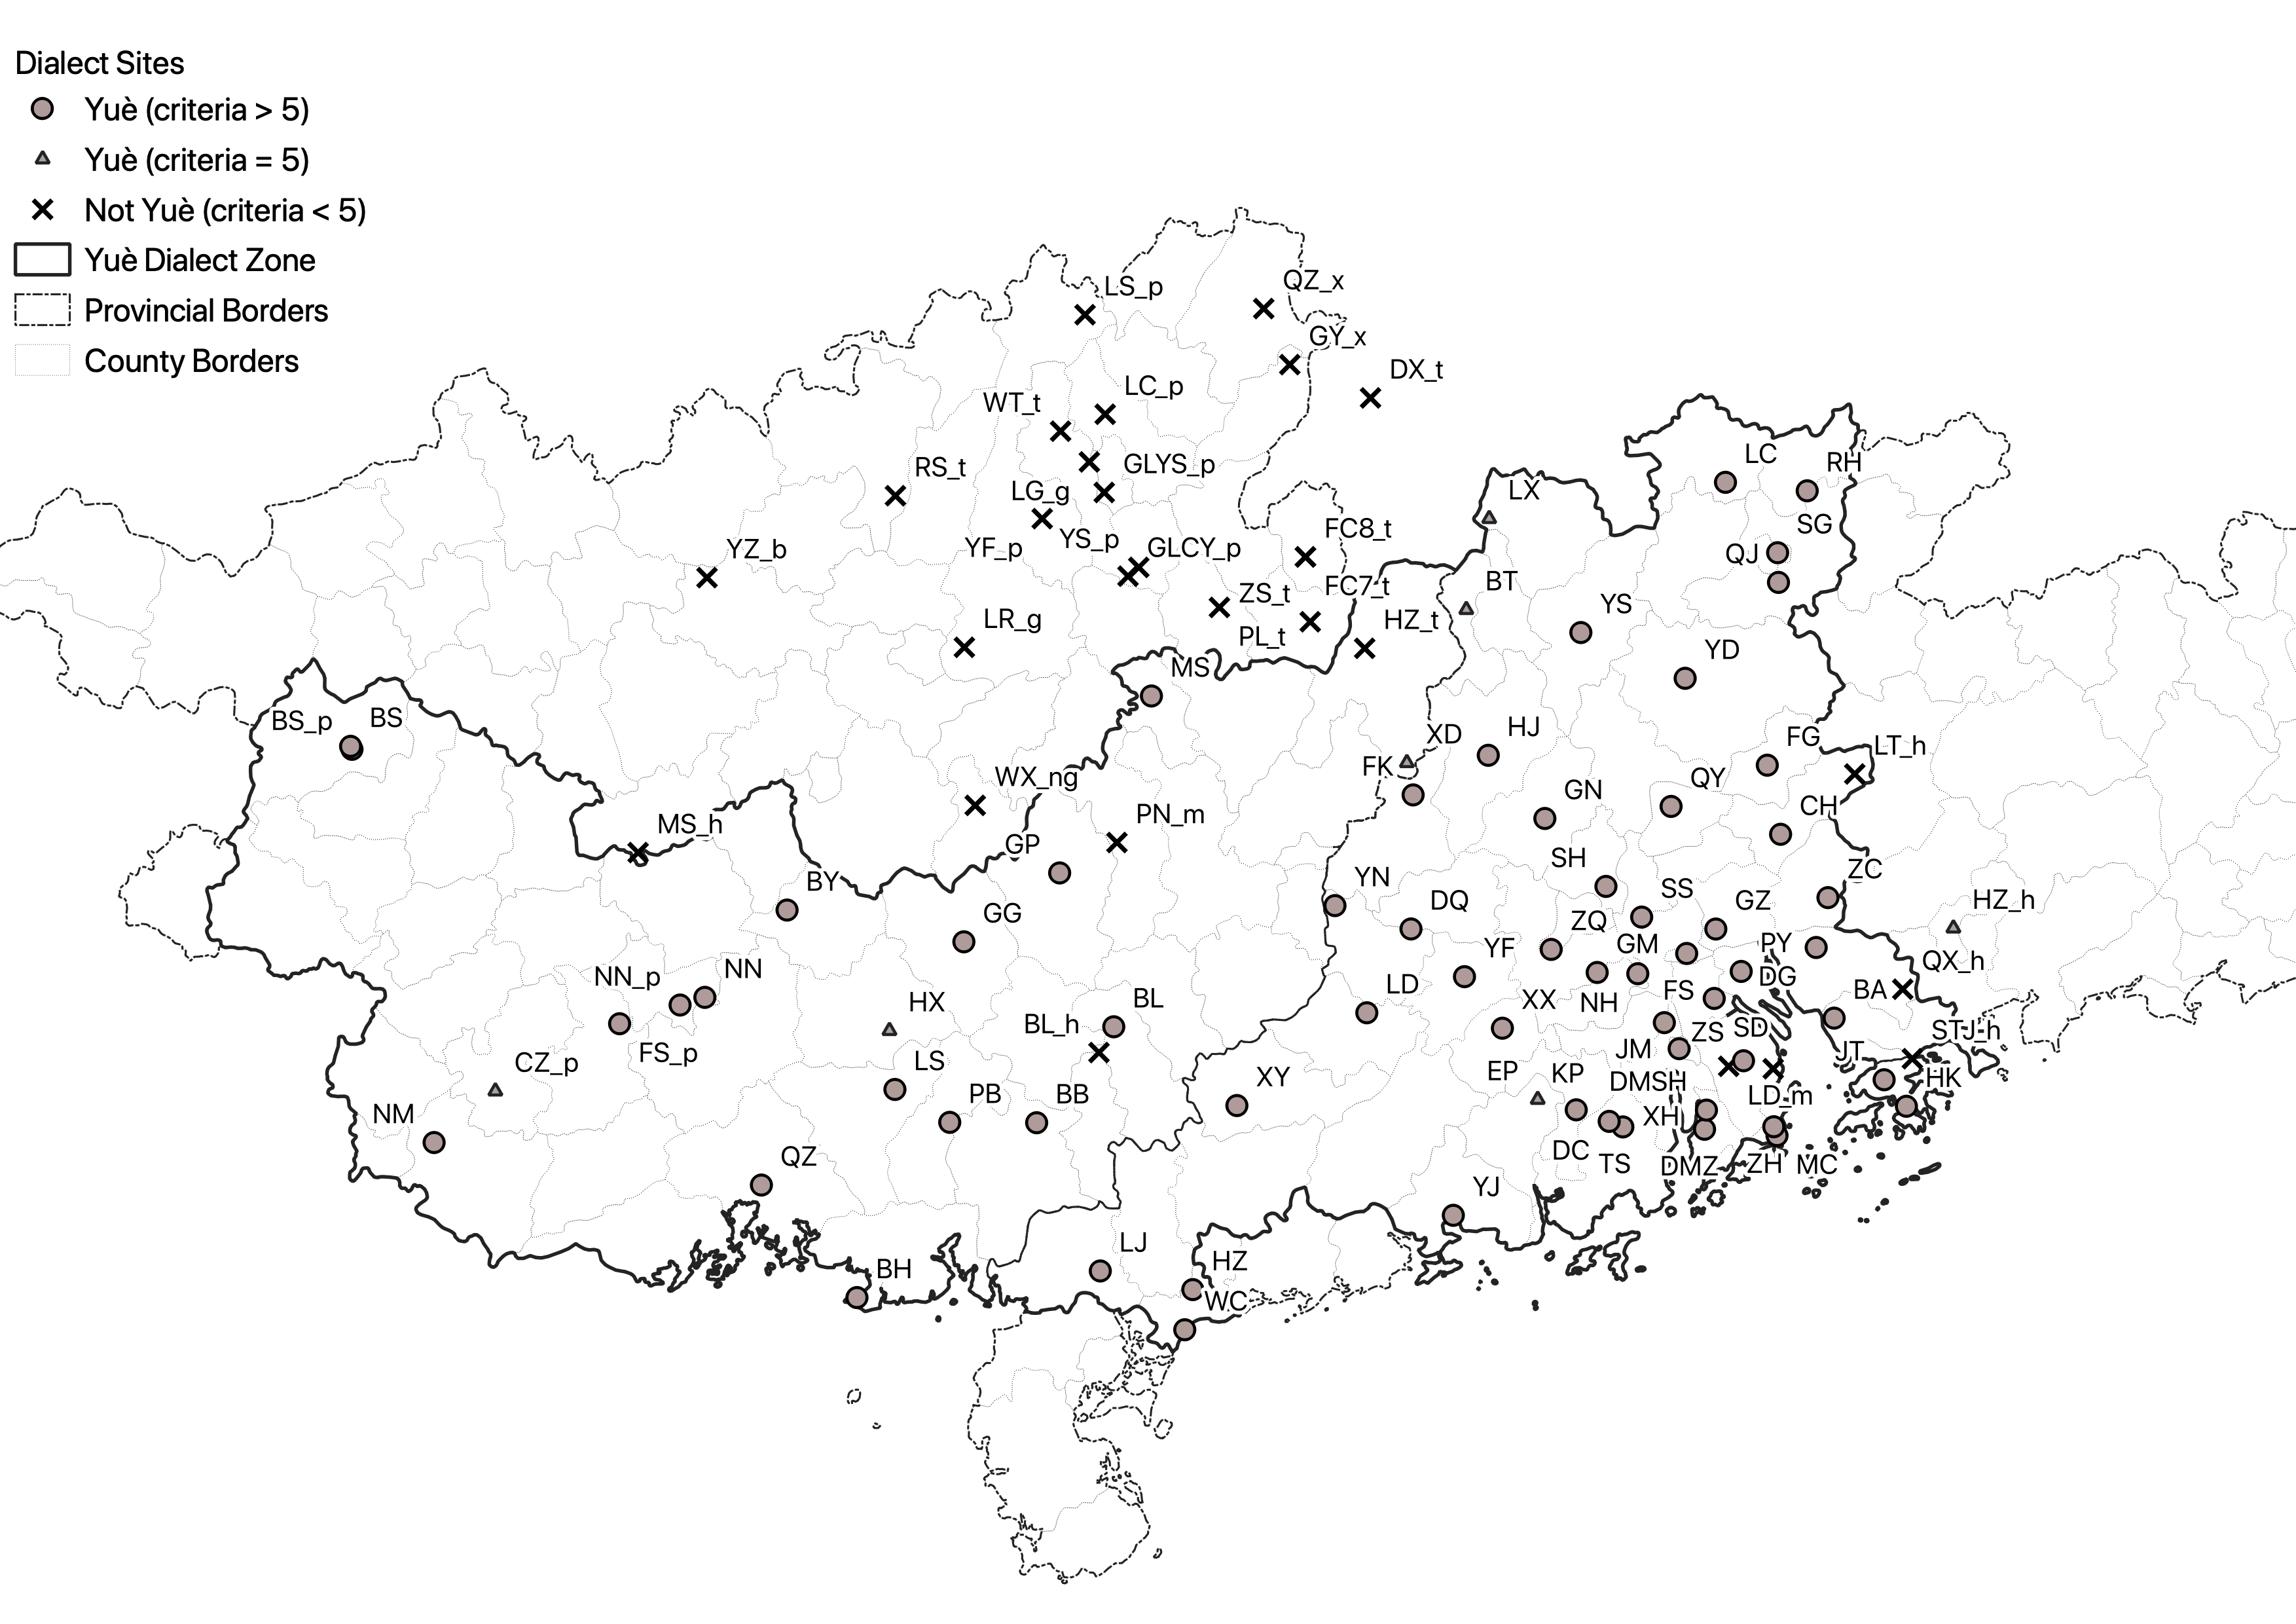
\includegraphics[width=.9\linewidth]{./cy_all_lex.png}
\caption{\label{fig:orgcbf50cd}The Diagnostic Applied to the Yuè Dialects and their Neighbors}
\end{figure}

\begin{itemize}
\item 5 or more -> (probably) Yuè Chinese
\item Convenient way to narrow focus to dialects most experts agree are Yuè. Not meant to be the final say.
\item Predicts S. Pinghua dialects are Yue, \emph{but} N. Pinghua dialects are not.
\end{itemize}



\newpage
\printbibliography
\end{document}